% \glsresetall
\chapter{Presentation of the results} % Main chapter title
\label{Chapter7}

\lhead{Chapter 7. \emph{Presentation of the results}}

In this chapter it will be explained how empirical traffic data was gathered using the prototype and which metrics were defined for comparison.
Afterwards the landscapes will be compared, using the defined metrics as key performance indicators. The actual evaluation of the results will be concluded in chapter \ref{Chapter8}.

\section{Data collection and metric definition} 

This section will contain information about how the data was collected and which metrics were defined based on the gathered data.

\subsection{Testing hardware and environment}

It has to be mentioned that certain aspects of the environment were not maintained by the tester and are therefore out of reach for influence or configuration. Nonetheless they are mentioned here for the sake of reproducibility.
The testing hardware and environment available were the following:

\begin{enumerate}
	\item \textbf{Laptop:}
	\begin{itemize}[noitemsep]
		\item MacBook Pro (15-inch, 2017)
		\item \textbf{Processor:} 2.9 GHz Quad-Core Intel Core i7
		\item \textbf{Memory:} 16 GB 2133 MHz LPDDR3 
		\item \textbf{Graphics:} Radeon Pro 560 4 GB and Intel HD Graphics 630 1536 MB
		\item \textbf{macOS Monetary - Version:} 12.2.1 (21D62)
	\end{itemize} 
	
	\item \textbf{Browser, Network and Lighthouse:}
	\begin{itemize}[noitemsep]
		\item \textbf{Browser:} Google Chrome
		\item \textbf{Version:} 99.0.4844.51 (Official Build) (x86\_64)
		\item \textbf{Chrome DevTools version:} Chrome 99
		\item \textbf{Lighthouse version:} 100.0.0.0
		\item \textbf{JavaScript version:} V8 9.9.115.8
		\item \textbf{Network-Bandwidth:} 180-200 MB/s
	\end{itemize}
	
	\item \textbf{Runtime environment for prototypes:} surge.sh \footnote{surge.sh is a platform for static web publishing
		for frontend developers via the command line.}
	
	\item \textbf{CDN:} Unpkg.com \footnote{This part of the environment was explained in chapter \ref{Chapter3}}
\end{enumerate}

Additionally to the specified hardware specs, version 1.18.1 of the \texttt{@luigi-project} was used. This dependency enables the Luigi framework and is therefore used in every implemented version of the prototype.

\subsection{Testing process}

Since multiple landscapes were implemented a unified process was required to collect comparable data. The BPMN diagram \ref{fig:data_collection_process_har} contains the process steps in detail.

\begin{figure}[!h]
	\centering
	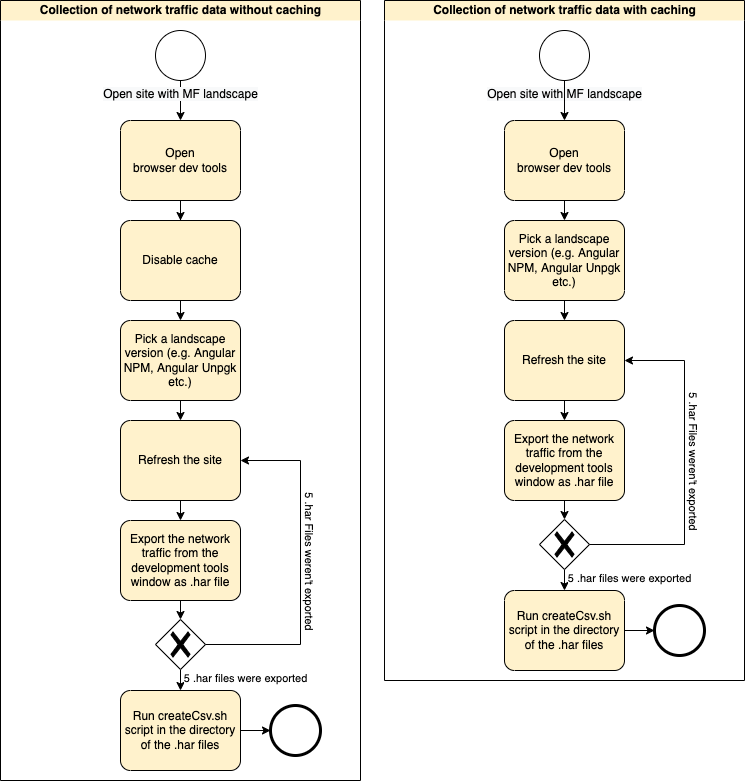
\includegraphics[width=0.7\textwidth]{Figures/Data_Collection_Process_har.drawio.png}
	\caption{Data collection process for .har files}
	\label{fig:data_collection_process_har}
\end{figure}

As it can be seen in \ref{fig:data_collection_process_har} there are actually two processes executed to collect data. The first one was with caching disabled, the second had it enabled. The intention behind it was to gather an average initial loading time for the picked side, therefore the resources must not be cached. 
The second process was used to gather information about caching behavior in general. Since each landscape contains basically the same views, the browser should be able to pull already loaded resources from the cache instead via the network. To showcase this behavior and prove the performance gain through caching, this data was gathered too.
Each process was executed 5 times, therefore 10 HTTP Archive (\texttt{.har}) files were generated per landscape. These \texttt{.har} files were then transformed into \texttt{.csv} files using a self-developed script. 

Additionally to the \texttt{.har} files a website performance report was collected, using the Lighthouse tool embedded in the Google Chrome browser. Such a report provides information about how much of the imported bytes are actually used by a web application, distinguished by resource URL.

In summary it means:

\begin{itemize}[noitemsep]
	\item 12 landscapes were developed
	\item Each landscape was loaded 10 times, 5 times with cache enabled and 5 with cache disabled
	\item Each loading of a landscape is represented by a HTTP Archive file
	\item In summary, the testing processes were executed 120 times overall
	\item Generating 120 \texttt{.har} files
	\item Which then were aggregated and transformed into 12 \texttt{.csv} files
	\item Which then again were copied into one Excel file, where the data was analyzed
	\item In addition 12 Lighthouse reports where collected (one per landscape) and added to the excel
\end{itemize}

The reason why this testing procedure was chosen was, due to the low variety in the parameters when a landscape was loaded. First it was tested if the parameters would vary when a landscape is loaded up to 1000 times, but that case did not occur. Due the constant resource sizes and stable network, not many fluctuations could be observed. Only when changes on technological level were made (e.g. usage of cache, network outage) fluctuations started to appeared. But other than that, it was observed that the results were stable. Therefore it was decided that loading a landscape 10 times does suffice for the experiment.

After the collection process, another self-developed script was used to aggregate all the gather data into one single file. This was later used to define and calculate the metrics, which are described next.

\subsection{Defined metrics}

The central file, containing all the data, was split into separate sheets in which the metrics for each micro frontend were calculated. The parameters for calculation were:

\begin{itemize}
	\item \textbf{connection} - This is an ID with which each opened TCP connection is tagged by the browser. This value can be an indicator for the parallelity of the requests. Since HTTP/2 several requests can be handled by a server via the same TCP connection, reducing the time costs for TCP handshakes. It has to be considered that the application requesting the sources can not implement this HTTP/2 feature. It has to be enabled on server side and by the browser, which is already the case for most modern browsers.\cite{http2} As of writing this transcript, Surge the web server platform, onto which the application landscapes are deployed, does not support HTTP/2.
	
	\item \textbf{loadedFromCache} - This is a string value with three possible characteristics, \textit{not loaded from cache, disk} or \textit{memory}, whereas \textit{disk} and \textit{memory} are semantically the same. This value explains from where the resource was loaded. Either via the network from a remote server or from the local cache. It helps indicating the caching behavior of bundled resources in comparison with resources loaded from a unified URL (e.g. a CDN). 
	
	\item \textbf{pageRef} - This is a page reference provided by the browser with possibly an infinite amount of characteristics. Each request is tagged with this value, so it can be distinguished, which request was sent by which web application. Since the data is separated by sheets inside the file and is always website specific, no further information can be pulled from this value.
	
	\item \textbf{startedDateTime} - This is a time stamp given to each request, marking its starting time in a DateTime format. This value can serve as an indicator for parallelity, since multiple TCP connections can be opened at the same time. 
	
	\item \textbf{requestMethod} - This is a string value with a limited amount of characteristics. The possible values are the different HTTP methods. It indicates which type of request was executed for the loaded resource. In almost all cases it is \textbf{GET}.
	
	\item \textbf{requestUrl} - This is a string value, containing the request URL used by the browser to load the resource. This value is mainly categorizing the calculation results, since neither \textit{connection} nor \textit{pageRef} are valid options to distinguish the loaded resources of a website. 
	
	\item \textbf{requestHeaderSize} - This is a number value, indicating the byte size of the request header sent by the web application to the server.
	
	\item \textbf{responseStatus} - This is a number value with a limited amount of characteristics, containing the HTTP response code from the server. The range of the possible values is the same as the possible response codes of the HTTP.
	
	\item \textbf{responseContentSize} - This number value is the byte size of the loaded resource.
	
	\item \textbf{timeInMs} - This value represents the round trip time of the request in milliseconds. 
\end{itemize}

Based on the given values from the \texttt{.har} files, following key performance indicators were calculated.

\begin{itemize}
	\item \textbf{Avg. Content Size} - Numerical value calculated by averaging the \textbf{responseContentSize} values of all the websites resources
	\item \textbf{Avg. Time in MS Loaded values} - Numerical value, calculated by averaging the \textbf{timeInMs} values of all the websites resources
	\item \textbf{Occurrences Connection Duplicates} - Numerical value to represent parallelity by counting the amount of duplicate/multiple occurring \textbf{connection} values
	\item \textbf{Connection IDs} - List of all \textbf{connection} characteristics for the website 
	\item \textbf{Connection IDs occurrence} - Amount of how often the connection occurred during the loading of the website
	\item \textbf{Parallel start time} - Numerical value, calculated by counting reoccurring \textbf{startedDateTime} values
	\item \textbf{Avg. Response content size per Loading Type} - Numerical value, calculated by averaging the \textbf{responseContentSize}, differentiated by the characteristics of the \textbf{loadedFromCache} property
	\item \textbf{URLs loaded} - List of all unique \textbf{requestUrl} values
	\item \textbf{Avg. Response Time per URL loaded in MS} - Numerical value, representing the average loading time of each loaded resource URL of the website
	\item \textbf{Avg. Response Size per URL loaded} - Numerical value, representing the average loading byte size of each resource URL
	\item \textbf{Avg. Response Size per URL loaded via network} - Numerical value, calculated by averaging the \textbf{responseContentSize} differentiated by the \textbf{requestUrl} for all resources with the \textbf{loadedFromCache} value of \textit{not loaded from cache}. For the test scenarios with cache disabled, this value equals \textbf{Avg. Response Size per URL loaded}
	\item \textbf{Avg. Response Size per URL loaded from Disk} - Numerical value, calculated by averaging the \textbf{responseContentSize} differentiated by the \textbf{requestUrl}, for all resources with the \textbf{loadedFromCache} value of \textit{disk}
	\item \textbf{Avg. Response Size per URL loaded from Memory} - Numerical value, calculated by averaging the \textbf{responseContentSize} differentiated by the \textbf{requestUrl}, for all resources with the \textbf{loadedFromCache} value of \textit{memory}
\end{itemize}

The main focus of this thesis is to reduce redundant libraries in micro frontend landscapes, by using different types of technologies. Therefore, the calculated metrics were used to partially determine the gain a technology brings. Nonetheless, it has to be considered, that certain indicators are hard to measure such as the complexity of the implemented technology.  
A metric like this, must not be ignored for the context of this transcript, since the gain or rather the value a technology brings, highly depends on it. Thus a subjective retrospective will be provided in chapter \ref{Chapter7}, describing the experience of the author with the used technologies.

In the following sections the results of the introduced metrics for each landscape are showcased. This display is distinguished by the fact, if the collected data was with caching enabled or not. Additionally to the metrics, the individual graphs for the landscapes are referred to in the appendixes \ref{appendix1}, \ref{appendix2} and \ref{appendix3}.

\section{CDN landscapes}

\subsection{Implementation with NPM}

The table \ref{tab:cdn_result_table} contains the results for the implemented landscapes with a regular bundler and a package manager, namely NPM. Certain metrics are not added to the table for readability, but a graphical representation can be found in \ref{appendix1}.

\scriptsize
\setlength{\mycolwidth}{\dimexpr \textwidth/5 - 2\tabcolsep}

\begin{longtable}[c]{*{3}{p{\mycolwidth}}}
	
	\caption{Table of numerical KPI results for the NPM landscapes with caching disabled}
	\label{tab:cdn_result_table} \\
	
	\toprule
	\multicolumn{1}{l}{\makecell[c]{\textbf{Metric}}}   
	& \multicolumn{1}{l}{\makecell[c]{\textbf{Angular NPM}}}                              
	& \multicolumn{1}{l}{\makecell[c]{\textbf{Vue NPM}}} \\ 
	\midrule
	\endfirsthead
	
	\multicolumn{3}{l}{\footnotesize\itshape\tablename~\thetable:
		continued from previous page} \\
	\toprule   
	\multicolumn{1}{l}{\makecell[c]{\textbf{Metric}}}   
	& \multicolumn{1}{l}{\makecell[c]{\textbf{Angular NPM}}}                              
	& \multicolumn{1}{l}{\makecell[c]{\textbf{Vue NPM}}} \\*
	\midrule
	\endhead
	%		
	\multicolumn{1}{l|}{URLs loaded count}                                         															
	& \multicolumn{1}{l|}{\makecell[c]{14}} 	
	& \multicolumn{1}{l}{\makecell[c]{13}}   \\ \midrule
	
	\multicolumn{1}{l|}{\makecell[l]{Avg. Response content size\\per Loading Type}}   
	& \multicolumn{1}{l|}{\makecell[c]{\textit{not loaded from cache} - 129529.13, \\ \textit{memory} - 0, \\ \textit{disk} - 0}} 											
	& \multicolumn{1}{l}{\makecell[c]{\textit{not loaded from cache} - 156131.63, \\ \textit{memory} - 0, \\ \textit{disk} - 0}}   \\ \midrule
	
	\multicolumn{1}{l|}{Parallel start time}                                 													
	& \multicolumn{1}{l|}{\makecell[c]{33}} 				
	& \multicolumn{1}{l}{\makecell[c]{45}}   \\ \midrule
	
	\multicolumn{1}{l|}{Connection IDs occurence}                            											
	& \multicolumn{1}{l|}{\makecell[c]{\textit{none established} - 10,\\ \textit{207393} - 10}} 												   
	& \multicolumn{1}{l}{\makecell[c]{\textit{241394} - 10}}   \\ \midrule
	
	\multicolumn{1}{l|}{Connection IDs count}                                      																
	& \multicolumn{1}{l|}{\makecell[c]{62}} 															     
	& \multicolumn{1}{l}{\makecell[c]{71}}   \\ \midrule
		
	\multicolumn{1}{l|}{\makecell[l]{Connection Duplicates}}                        
	& \multicolumn{1}{l|}{\makecell[c]{20}} 						   
	& \multicolumn{1}{l}{\makecell[c]{10}}   \\ \midrule
	
	\multicolumn{1}{l|}{\makecell[l]{Loaded values \& occurrences}}                        
	& \multicolumn{1}{c|}{\makecell[c]{\textit{not loaded from cache} - 80,\\ \textit{memory} - 0, \\ \textit{disk} - 0}} 						   
	& \multicolumn{1}{l}{\makecell[c]{\textit{not loaded from cache} - 80, \\ \textit{memory} - 0, \\ \textit{disk} - 0}}   \\ \midrule
	
	\multicolumn{1}{l|}{\makecell[l]{Avg. Time in MS}}                        
	& \multicolumn{1}{l|}{\makecell[c]{162.22}} 						   
	& \multicolumn{1}{l}{\makecell[c]{5323.54}}   \\ \midrule
	
	\multicolumn{1}{l|}{\makecell[l]{Avg. Content Size}}                                         
	& \multicolumn{1}{l|}{\makecell[c]{129529.13}}  				  
	&   \multicolumn{1}{l}{\makecell[c]{156131.63}} \\ \bottomrule
\end{longtable}

\normalsize
The results shown in table \ref{tab:cdn_result_table} were collected without caching enabled. This explains for instance, why no resources were loaded from cache and therefore the values for the \textit{memory} or \textit{disk} characteristics are missing.
The main takeaway from these results, is an average initial loading time for the landscapes which range from \textbf{129529.125} to \textbf{156131.625} milliseconds, depending on the framework. It can also be seen, that even though less resources are loaded via URLs by the VueJS landscape, it has a longer loading time compared to the Angular one.

\scriptsize
\setlength{\mycolwidth}{\dimexpr \textwidth/5 - 2\tabcolsep}

\begin{longtable}[c]{*{3}{p{\mycolwidth}}}
	
	\caption{Table of numerical KPI results for the NPM landscapes with caching enabled}
	\label{tab:cdn_result_table_caching} \\
	
	\toprule
	\multicolumn{1}{l}{\makecell[c]{\textbf{Metric}}}   
	& \multicolumn{1}{l}{\makecell[c]{\textbf{Angular NPM}}}                              
	& \multicolumn{1}{l}{\makecell[c]{\textbf{Vue NPM}}} \\ 
	\midrule
	\endfirsthead
	
	\multicolumn{3}{l}{\footnotesize\itshape\tablename~\thetable:
		continued from previous page} \\
	\toprule   
	\multicolumn{1}{l}{\makecell[c]{\textbf{Metric}}}   
	& \multicolumn{1}{l}{\makecell[c]{\textbf{Angular NPM}}}                              
	& \multicolumn{1}{l}{\makecell[c]{\textbf{Vue NPM}}} \\*
	\midrule
	\endhead
	%		
	\multicolumn{1}{l|}{URLs loaded count}                                         															
	& \multicolumn{1}{l|}{\makecell[c]{14}} 	
	& \multicolumn{1}{l}{\makecell[c]{13}}   \\ \midrule
	
	\multicolumn{1}{l|}{\makecell[l]{Avg. Response content size\\per Loading Type}}   
	& \multicolumn{1}{l|}{\makecell[c]{\textit{not loaded from cache} - 166856, \\ \textit{memory} - 17548.5, \\ \textit{disk} - 17548.5}} 											
	& \multicolumn{1}{l}{\makecell[c]{\textit{not loaded from cache} - 145646.67,\\ \textit{memory} - 0, \\ \textit{disk} - 187586.5}}   \\ \midrule
	
	\multicolumn{1}{l|}{Parallel start time}                                 													
	& \multicolumn{1}{l|}{\makecell[c]{32}} 				
	& \multicolumn{1}{l}{\makecell[c]{39}}   \\ \midrule
	
	\multicolumn{1}{l|}{Connection IDs occurence}                            											
	& \multicolumn{1}{l|}{\makecell[c]{\textit{none established} - 20}} 												   
	& \multicolumn{1}{l}{\makecell[c]{\textit{none established} - 20}}   \\ \midrule
	
	\multicolumn{1}{l|}{Connection IDs count}                                      																
	& \multicolumn{1}{l|}{\makecell[c]{61}} 															     
	& \multicolumn{1}{l}{\makecell[c]{61}}   \\ \midrule
	
	\multicolumn{1}{l|}{\makecell[l]{Connection Duplicates}}                        
	& \multicolumn{1}{l|}{\makecell[c]{20}} 						   
	& \multicolumn{1}{l}{\makecell[c]{20}}   \\ \midrule
	
	\multicolumn{1}{l|}{\makecell[l]{Loaded values \& occurrences}}                        
	& \multicolumn{1}{c|}{\makecell[c]{\textit{not loaded from cache} - 60, \\ \textit{memory} - 6, \\ \textit{disk} - 14}} 						   
	& \multicolumn{1}{l}{\makecell[c]{\textit{not loaded from cache} - 60, \\ \textit{memory} - 0, \\ \textit{disk} - 20}}   \\ \midrule
	
	\multicolumn{1}{l|}{\makecell[l]{Avg. Time in MS}}                        
	& \multicolumn{1}{l|}{\makecell[c]{150.90}} 						   
	& \multicolumn{1}{l}{\makecell[c]{1890.6}}   \\ \midrule
	
	\multicolumn{1}{l|}{\makecell[l]{Avg. Content Size}}                                         
	& \multicolumn{1}{l|}{\makecell[c]{129529.13}}  				  
	&   \multicolumn{1}{l}{\makecell[c]{156131.63}} \\ \bottomrule
	
\end{longtable}

\normalsize
The results of table \ref{tab:cdn_result_table_caching} show the effect caching has on the performance of a site. The average loading time of the site decreases, as do the opened TCP connections. In table \ref{cdn_result_table}, the Angular landscape is loaded faster compared to Vue JS.

Both environments were implemented using a regular bundler and therefore it can not be ensured that redundant libraries were not loaded.

\subsection{Implementation with Unpkg}

Table \ref{tab:cdn_result_table_unpkg} contains the results for the implemented landscapes with a use of a public CDN, namely Unpkg. Certain metrics are not added to the table for readability, but a graphical representation can be found in \ref{appendix1}. 

\scriptsize
\setlength{\mycolwidth}{\dimexpr \textwidth/5 - 2\tabcolsep}

\begin{longtable}[c]{*{3}{p{\mycolwidth}}}
	
	\caption{Table of numerical KPI results for the landscapes using the Unpkg CDN with caching disabled}
	\label{tab:cdn_result_table_unpkg} \\
	
	\toprule
	\multicolumn{1}{l}{\makecell[c]{\textbf{Metric}}}   
	& \multicolumn{1}{l}{\makecell[c]{\textbf{Angular Unpkg}}}                              
	& \multicolumn{1}{l}{\makecell[c]{\textbf{Vue Unpkg}}} \\ 
	\midrule
	\endfirsthead
	
	\multicolumn{3}{l}{\footnotesize\itshape\tablename~\thetable:
		continued from previous page} \\
	\toprule                        
	\multicolumn{1}{l}{\makecell[c]{\textbf{Metric}}}   
	& \multicolumn{1}{l}{\makecell[c]{\textbf{Angular Unpkg}}}                              
	& \multicolumn{1}{l}{\makecell[c]{\textbf{Vue Unpkg}}} \\*
	\midrule
	\endhead
	%		
	\multicolumn{1}{l|}{URLs loaded count}                                         															
	& \multicolumn{1}{l|}{\makecell[c]{171}} 	
	& \multicolumn{1}{l}{\makecell[c]{165}}   \\ \midrule
	
	\multicolumn{1}{l|}{\makecell[l]{Avg. Response content size\\per Loading Type}}   
	& \multicolumn{1}{l|}{\makecell[c]{\textit{not loaded from cache} - 9768.62, \\ \textit{memory} - 0, \\ \textit{disk} - 0}} 											
	& \multicolumn{1}{l}{\makecell[c]{\textit{not loaded from cache} - 8205.19, \\ \textit{memory} - 0, \\ \textit{disk} - 0}}   \\ \midrule
	
	\multicolumn{1}{l|}{Parallel start time}                                 													
	& \multicolumn{1}{l|}{\makecell[c]{871}} 				
	& \multicolumn{1}{l}{\makecell[c]{989}}   \\ \midrule
	
	\multicolumn{1}{l|}{Connection IDs occurence}                            											
	& \multicolumn{1}{l|}{\makecell[c]{\textit{223736} - 20,\\ \textit{223722} - 1574,\\ \textit{none established} - 10}} 												   
	& \multicolumn{1}{l}{\makecell[c]{\textit{241394} - 20,\\ \textit{249654} - 1560}}   \\ \midrule
	
	\multicolumn{1}{l|}{Connection IDs count}                                      																
	& \multicolumn{1}{l|}{\makecell[c]{53}} 															     
	& \multicolumn{1}{l}{\makecell[c]{42}}   \\ \midrule
	
	\multicolumn{1}{l|}{\makecell[l]{Connection Duplicates}}                        
	& \multicolumn{1}{l|}{\makecell[c]{1604}} 						   
	& \multicolumn{1}{l}{\makecell[c]{1580}}   \\ \midrule
	
	\multicolumn{1}{l|}{\makecell[l]{Loaded values \&\\ occurrences}}                        
	& \multicolumn{1}{c|}{\makecell[c]{\textit{not loaded from cache} - 1654, \\ \textit{memory} - 0, \\ \textit{disk} - 0}} 						   
	& \multicolumn{1}{l}{\makecell[c]{\textit{not loaded from cache} - 1620, \\ \textit{memory} - 0, \\ \textit{disk} - 0}}   \\ \midrule
	
	\multicolumn{1}{l|}{\makecell[l]{Avg. Time in MS}}                        
	& \multicolumn{1}{l|}{\makecell[c]{97.23}} 						   
	& \multicolumn{1}{l}{\makecell[c]{194.01}}   \\ \midrule
	
	\multicolumn{1}{l|}{\makecell[l]{Avg. Content Size}}                                         
	& \multicolumn{1}{l|}{\makecell[c]{9768.62}}  				  
	&   \multicolumn{1}{l}{\makecell[c]{8205.19}} \\ \bottomrule
	
\end{longtable}

\normalsize
The data shown in table \ref{tab:cdn_result_table_unpkg} are again collected without caching enabled. An approximate estimation for the initial loading times can be drawn from this. It is made visible that the VueJS environment takes longer to load for less content. A similar behavior was present in the NPM implementation.
Nonetheless it is an improvement in performance compared to the NPM counterparts for both landscapes. The trade-off of this technology is that single component resources, like a button or a table, were imported via script tags one by one, thus the increase in loaded URLs.

\scriptsize
\setlength{\mycolwidth}{\dimexpr \textwidth/5 - 2\tabcolsep}

\begin{longtable}[c]{*{3}{p{\mycolwidth}}}
 	
 	\caption{Table of numerical KPI results for the landscapes using the Unpkg CDN with caching enabled}
 	\label{tab:cdn_result_table_unpkg_cache} \\
 	
 	\toprule
	\multicolumn{1}{l}{\makecell[c]{\textbf{Metric}}}   
	& \multicolumn{1}{l}{\makecell[c]{\textbf{Angular Unpkg}}}                              
	& \multicolumn{1}{l}{\makecell[c]{\textbf{Vue Unpkg}}} \\ 
 	\midrule
 	\endfirsthead
 	
 	\multicolumn{3}{l}{\footnotesize\itshape\tablename~\thetable:
 		continued from previous page} \\
 	\toprule   
	\multicolumn{1}{l}{\makecell[c]{\textbf{Metric}}}   
	& \multicolumn{1}{l}{\makecell[c]{\textbf{Angular Unpkg}}}                              
	& \multicolumn{1}{l}{\makecell[c]{\textbf{Vue Unpkg}}} \\*
 	\midrule
 	\endhead
 	%		
 	\multicolumn{1}{l|}{URLs loaded count}                                         															
 	& \multicolumn{1}{l|}{\makecell[c]{171}} 	
 	& \multicolumn{1}{l}{\makecell[c]{165}}   \\ \midrule
 	
 	\multicolumn{1}{l|}{\makecell[l]{Avg. Response content size\\per Loading Type}}   
 	& \multicolumn{1}{l|}{\makecell[c]{\textit{not loaded from cache} - 63972.08, \\ \textit{memory} - 208838, \\ \textit{disk} - 7166.1}} 											
 	& \multicolumn{1}{l}{\makecell[c]{\textit{not loaded from cache} - 28143.2, \\ \textit{memory} - 0, \\ \textit{disk} - 7570.22}}   \\ \midrule
 	
 	\multicolumn{1}{l|}{Parallel start time}                                 													
 	& \multicolumn{1}{l|}{\makecell[c]{1111}} 				
 	& \multicolumn{1}{l}{\makecell[c]{1069}}   \\ \midrule
 	
 	\multicolumn{1}{l|}{Connection IDs occurence}                            											
 	& \multicolumn{1}{l|}{\makecell[c]{\textit{none established} - 1590,\\ \textit{223722} - 15}} 												   
 	& \multicolumn{1}{l}{\makecell[c]{\textit{none established} - 1570,\\ \textit{249654} - 10}}   \\ \midrule
 	
 	\multicolumn{1}{l|}{Connection IDs count}                                      																
 	& \multicolumn{1}{l|}{\makecell[c]{52}} 															     
 	& \multicolumn{1}{l}{\makecell[c]{42}}   \\ \midrule
 	
 	\multicolumn{1}{l|}{\makecell[l]{Connection Duplicates}}                        
 	& \multicolumn{1}{l|}{\makecell[c]{1605}} 						   
 	& \multicolumn{1}{l}{\makecell[c]{1580}}   \\ \midrule
 	
 	\multicolumn{1}{l|}{\makecell[l]{Loaded values \& occurrences}}                        
 	& \multicolumn{1}{c|}{\makecell[c]{\textit{not loaded from cache} - 65, \\ \textit{memory} - 3, \\ \textit{disk} - 1587}} 						   
 	& \multicolumn{1}{l}{\makecell[c]{\textit{not loaded from cache} - 50, \\ \textit{memory} - 0, \\ \textit{disk} - 1570}}   \\ \midrule
 	
 	\multicolumn{1}{l|}{\makecell[l]{Avg. Time in MS}}                        
 	& \multicolumn{1}{l|}{\makecell[c]{58.73}} 						   
 	& \multicolumn{1}{l}{\makecell[c]{87.1}}   \\ \midrule
 	
 	\multicolumn{1}{l|}{\makecell[l]{Avg. Content Size}}                                         
 	& \multicolumn{1}{l|}{\makecell[c]{9762.72}}  				  
 	&   \multicolumn{1}{l}{\makecell[c]{8205.19}} \\ \bottomrule
 	
\end{longtable}

\normalsize
A similar development can be observed in table \ref{tab:cdn_result_table_unpkg_cache} as previously. Primarily with caching enabled, the average loading times decrease, secondly the amount of loaded resources from cache increases significantly and lastly the Angular environments show shorter average loading times despite more resources were requested by them.

\section{Web Components/Compound and WMF landscapes}

As the described in chapter \ref{Chapter6}, these environments exist in different versions. They were designed that way to showcase how the used technologies handle multi-version landscapes and how they affect the performance.
Table \ref{tab:wmf_compound} shows the above mentioned KPIs of those environments.
 

\scriptsize
\setlength{\mycolwidth}{\dimexpr \textwidth/5 - 2\tabcolsep}

\begin{longtable}[c]{*{3}{p{\mycolwidth}}}
	
	\caption{Table of numerical KPI results for the landscapes implemented with Web Components as compound views and WMF with caching disabled}
	\label{tab:wmf_compound} \\
	
	\toprule
	\multicolumn{1}{l}{\makecell[c]{\textbf{Metric}}}   
	& \multicolumn{1}{l}{\makecell[c]{\textbf{WC/Compound}}}                              
	& \multicolumn{1}{l}{\makecell[c]{\textbf{WMF}}} \\ 
	\midrule
	\endfirsthead
	
	\multicolumn{3}{l}{\footnotesize\itshape\tablename~\thetable: continued from previous page} \\
	\toprule                        
	\multicolumn{1}{l}{\makecell[c]{\textbf{Metric}}}   
	& \multicolumn{1}{l}{\makecell[c]{\textbf{WC/Compound }}}                              
	& \multicolumn{1}{l}{\makecell[c]{\textbf{WMF}}} \\*
	\midrule
	\endhead
	%		
	\multicolumn{1}{l|}{URLs loaded count}                                         															
	& \multicolumn{1}{l|}{\makecell[c]{27}} 	       
	& \multicolumn{1}{l}{\makecell[c]{118}}   \\ \midrule
	
	\multicolumn{1}{l|}{\makecell[l]{Avg. Response content size\\per Loading Type}}   
	& \multicolumn{1}{l|}{\makecell[c]{\textit{not loaded from cache} - 213266.74, \\ \textit{memory} - 0,\\ \textit{disk} - 0}} 			         
	& \multicolumn{1}{l}{\makecell[c]{\textit{not loaded from cache} - 507168.76, \\ \textit{memory} - 0, \\ \textit{disk} - 0}}   \\ \midrule
	
	\multicolumn{1}{l|}{Parallel start time}                                 													
	& \multicolumn{1}{l|}{\makecell[c]{29}} 				                  
	& \multicolumn{1}{l}{\makecell[c]{109}}   \\ \midrule
	
	\multicolumn{1}{l|}{Connection IDs occurence}                            											
	& \multicolumn{1}{l|}{\makecell[c]{\textit{78725} - 15,\\ \textit{78890} - 15}} 		              
	& \multicolumn{1}{l}{\makecell[c]{\textit{728247} - 3,\\ \textit{none established} - 14}}   \\ \midrule
	
	\multicolumn{1}{l|}{Connection IDs count}                                      																
	& \multicolumn{1}{l|}{\makecell[c]{546}} 		         											     
	& \multicolumn{1}{l}{\makecell[c]{42}}   \\ \midrule
	
	\multicolumn{1}{l|}{\makecell[l]{Connection Duplicates}}                        
	& \multicolumn{1}{l|}{\makecell[c]{30}} 					
	& \multicolumn{1}{l}{\makecell[c]{20}}   \\ \midrule
	
	\multicolumn{1}{l|}{\makecell[l]{Loaded values \& occurrences}}                          
	& \multicolumn{1}{c|}{\makecell[c]{\textit{not loaded from cache} - 135, \\ \textit{memory} - 30, \\ \textit{disk} - 0}} 						   
	& \multicolumn{1}{l}{\makecell[c]{\textit{not loaded from cache} - 563, \\ \textit{memory} - 0, \\ \textit{disk} - 0}}   \\ \midrule
	
	\multicolumn{1}{l|}{\makecell[l]{Avg. Time in MS}}                        
	& \multicolumn{1}{l|}{\makecell[c]{2454.95}} 	                			   
	& \multicolumn{1}{l}{\makecell[c]{552.7}}   \\ \midrule
	
	\multicolumn{1}{l|}{\makecell[l]{Avg. Content Size}}                                         
	& \multicolumn{1}{l|}{\makecell[c]{213266.74}}  		          
	&   \multicolumn{1}{l}{\makecell[c]{507168.76}} \\ \bottomrule
	
\end{longtable}

\normalsize
As the data in table \ref{tab:wmf_compound} shows, the initial loading time for the Compound/Web Components environments is significantly lower compared to the WMF counterpart. Also the amount of loaded resources differs. This is due to the fact, that WMF has to be used in combination with the Webpack 5 bundler. Therefore certain resources might be loaded several times, if not configured as shared dependencies in the Module Federation. 
Table \ref{tab:wmf_compound_cache} showcases the same landscapes, but with caching enabled.

\scriptsize
\setlength{\mycolwidth}{\dimexpr \textwidth/5 - 2\tabcolsep}

\begin{longtable}[c]{*{3}{p{\mycolwidth}}}
	
	\caption{Table of numerical KPI results for the landscapes implemented with Web Components as compound views and WMF with caching enabled}
	\label{tab:wmf_compound_cache} \\
	
	\toprule
	\multicolumn{1}{l}{\makecell[c]{\textbf{Metric}}}   
	& \multicolumn{1}{l}{\makecell[c]{\textbf{WC/Compound}}}                              
	& \multicolumn{1}{l}{\makecell[c]{\textbf{WMF}}} \\ 
	\midrule
	\endfirsthead
	
	\multicolumn{3}{l}{\footnotesize\itshape\tablename~\thetable: continued from previous page} \\
	\toprule                        
	\multicolumn{1}{l}{\makecell[c]{\textbf{Metric}}}   
	& \multicolumn{1}{l}{\makecell[c]{\textbf{WC/Compound}}}                              
	& \multicolumn{1}{l}{\makecell[c]{\textbf{WMF}}} \\*
	\midrule
	\endhead
	%		
	\multicolumn{1}{l|}{URLs loaded count}                                         															
	& \multicolumn{1}{l|}{\makecell[c]{27}} 	       
	& \multicolumn{1}{l}{\makecell[c]{109}}   \\ \midrule
	
	\multicolumn{1}{l|}{\makecell[l]{Avg. Response content size\\per Loading Type}}   
	& \multicolumn{1}{l|}{\makecell[c]{\textit{not loaded from cache} - 215385.36, \\ \textit{memory} - 167973, \\ \textit{disk} - 588082}} 			         
	& \multicolumn{1}{l}{\makecell[c]{\textit{not loaded from cache} - 525243.08, \\ \textit{memory} - 0, \\ \textit{disk} - 1959}}   \\ \midrule
	
	\multicolumn{1}{l|}{Parallel start time}                                 													
	& \multicolumn{1}{l|}{\makecell[c]{35}} 				                  
	& \multicolumn{1}{l}{\makecell[c]{105}}   \\ \midrule
	
	\multicolumn{1}{l|}{Connection IDs occurence}                            											
	& \multicolumn{1}{l|}{\makecell[c]{\textit{none established} - 4,\\ \textit{78890} - 15,\\ \textit{78725} - 11}} 		              
	& \multicolumn{1}{l}{\makecell[c]{\textit{none established} - 15}}   \\ \midrule
	
	\multicolumn{1}{l|}{Connection IDs count}                                      																
	& \multicolumn{1}{l|}{\makecell[c]{104}} 		         											     
	& \multicolumn{1}{l}{\makecell[c]{537}}   \\ \midrule
	
	\multicolumn{1}{l|}{\makecell[l]{Connection Duplicates}}                        
	& \multicolumn{1}{l|}{\makecell[c]{30}} 					
	& \multicolumn{1}{l}{\makecell[c]{15}}   \\ \midrule
	
	\multicolumn{1}{l|}{\makecell[l]{Loaded values \& occurrences}}                          
	& \multicolumn{1}{c|}{\makecell[c]{\textit{not loaded from cache} - 107, \\ \textit{memory} - 20, \\ \textit{disk} - 4}} 						   
	& \multicolumn{1}{l}{\makecell[c]{\textit{not loaded from cache} - 536, \\ \textit{memory} - 0, \\ \textit{disk} - 15}}   \\ \midrule
	
	\multicolumn{1}{l|}{\makecell[l]{Avg. Time in MS}}                        
	& \multicolumn{1}{l|}{\makecell[c]{897.62}} 	                			   
	& \multicolumn{1}{l}{\makecell[c]{356.53}}   \\ \midrule
	
	\multicolumn{1}{l|}{\makecell[l]{Avg. Content Size}}                                         
	& \multicolumn{1}{l|}{\makecell[c]{219526.89}}  		          
	&   \multicolumn{1}{l}{\makecell[c]{510997.6}} \\ \bottomrule
	
\end{longtable}

\normalsize
The results with the caching enabled are not so different compared to the disabled caching ones. For instances, in both cases the average loading time for the compound landscape has longer loading times for fewer resources. One aspect differs though, compared to the compound landscape the WMF one has little cached resources. Also it becomes visible that the average content size loaded is smaller. Therefore, the Lighthouse tool was used to gather further information and data about those applications. The next section will showcase and explain the analysis done.

\section{Lighthouse analysis}

It has to be mentioned in advance that the following data is considered to be representative. Therefore, it is assumed that similar landscapes would follow a similar result in general. Nonetheless it is possible that for single cases the reports differ, since the within lying calculations are highly application dependent.
For the sake of completeness the reports are shown below.

The given data was gathered based on the previously introduced landscapes. It contains the analysis of the imported resources and how much of the corresponding imports were not used by the application, measured in bytes. First a tabular view is provided, following by the corresponding graph.

\newpage

\scriptsize 
\setlength{\mycolwidthtwo}{\dimexpr \textwidth/5 - 2\tabcolsep}%

\begin{longtable}[c]{*{4}{p{\mycolwidthtwo}}}
	
	\caption{Table of the average imported and unused bytes values, collected via the Lighthouse tool in the prototype landscapes}
	\label{tab:lighthouse_used_report} \\
	
	\toprule
	\textbf{Landscape}                        
	& \multicolumn{1}{l}{\makecell[c]{\textbf{Avg. imported bytes}}}   
	& \multicolumn{1}{l}{\makecell[c]{\textbf{Avg. unused bytes}}}                              
	& \multicolumn{1}{l}{\makecell[c]{\textbf{Avg. unused bytes in \%}}} \\                                    
	\midrule
	\endfirsthead
	
	\multicolumn{4}{l}{\footnotesize\itshape\tablename~\thetable: continued from previous page} \\
	\toprule        
	\textbf{Landscape}                        
	& \multicolumn{1}{l}{\makecell[c]{\textbf{Avg. imported bytes}}}   
	& \multicolumn{1}{l}{\makecell[c]{\textbf{Avg. unused bytes}}}                              
	& \multicolumn{1}{l}{\makecell[c]{\textbf{Avg. unused bytes in \%}}} \\*
	\midrule
	\endhead
	%		
	\multicolumn{1}{l|}{Angular NPM}                                         															
	& \multicolumn{1}{l|}{\makecell[c]{219257.14}} 	       
	& \multicolumn{1}{l|}{\makecell[c]{93671.43}}   
	& \multicolumn{1}{l}{\makecell[c]{42.72}} 	\\ \midrule
		
	\multicolumn{1}{l|}{Angular Unpkg}                                 													
	& \multicolumn{1}{l|}{\makecell[c]{13126.84}} 				                  
	& \multicolumn{1}{l|}{\makecell[c]{7425.87}}   
	& \multicolumn{1}{l}{\makecell[c]{56.57}} \\ \midrule
	
	\multicolumn{1}{l|}{Vue NPM}                            											
	& \multicolumn{1}{l|}{\makecell[c]{281262.33}} 		              
	& \multicolumn{1}{l|}{\makecell[c]{123902}}    
	& \multicolumn{1}{l}{\makecell[c]{44.05}} \\ \midrule
	
	\multicolumn{1}{l|}{Vue Unpkg}                                      																
	& \multicolumn{1}{l|}{\makecell[c]{12057.91}} 		         											     
	& \multicolumn{1}{l|}{\makecell[c]{6844.21}}    
	& \multicolumn{1}{l}{\makecell[c]{56.76}} \\ \midrule
	
	\multicolumn{1}{l|}{\makecell[l]{Compound/\\Web Components}}                        
	& \multicolumn{1}{l|}{\makecell[c]{229483.67}} 					
	& \multicolumn{1}{l|}{\makecell[c]{90265.19}}    
	& \multicolumn{1}{l}{\makecell[c]{39.33}} \\ \midrule
	
	\multicolumn{1}{l|}{\makecell[l]{Webpack\\Module\\Federation}}                         
	& \multicolumn{1}{l|}{\makecell[c]{551111.19}} 						   
	& \multicolumn{1}{l|}{\makecell[c]{222113.73}}   
	& \multicolumn{1}{l}{\makecell[c]{40.31}}  \\ \midrule
\end{longtable}

\begin{figure}[!h]
	\centering
	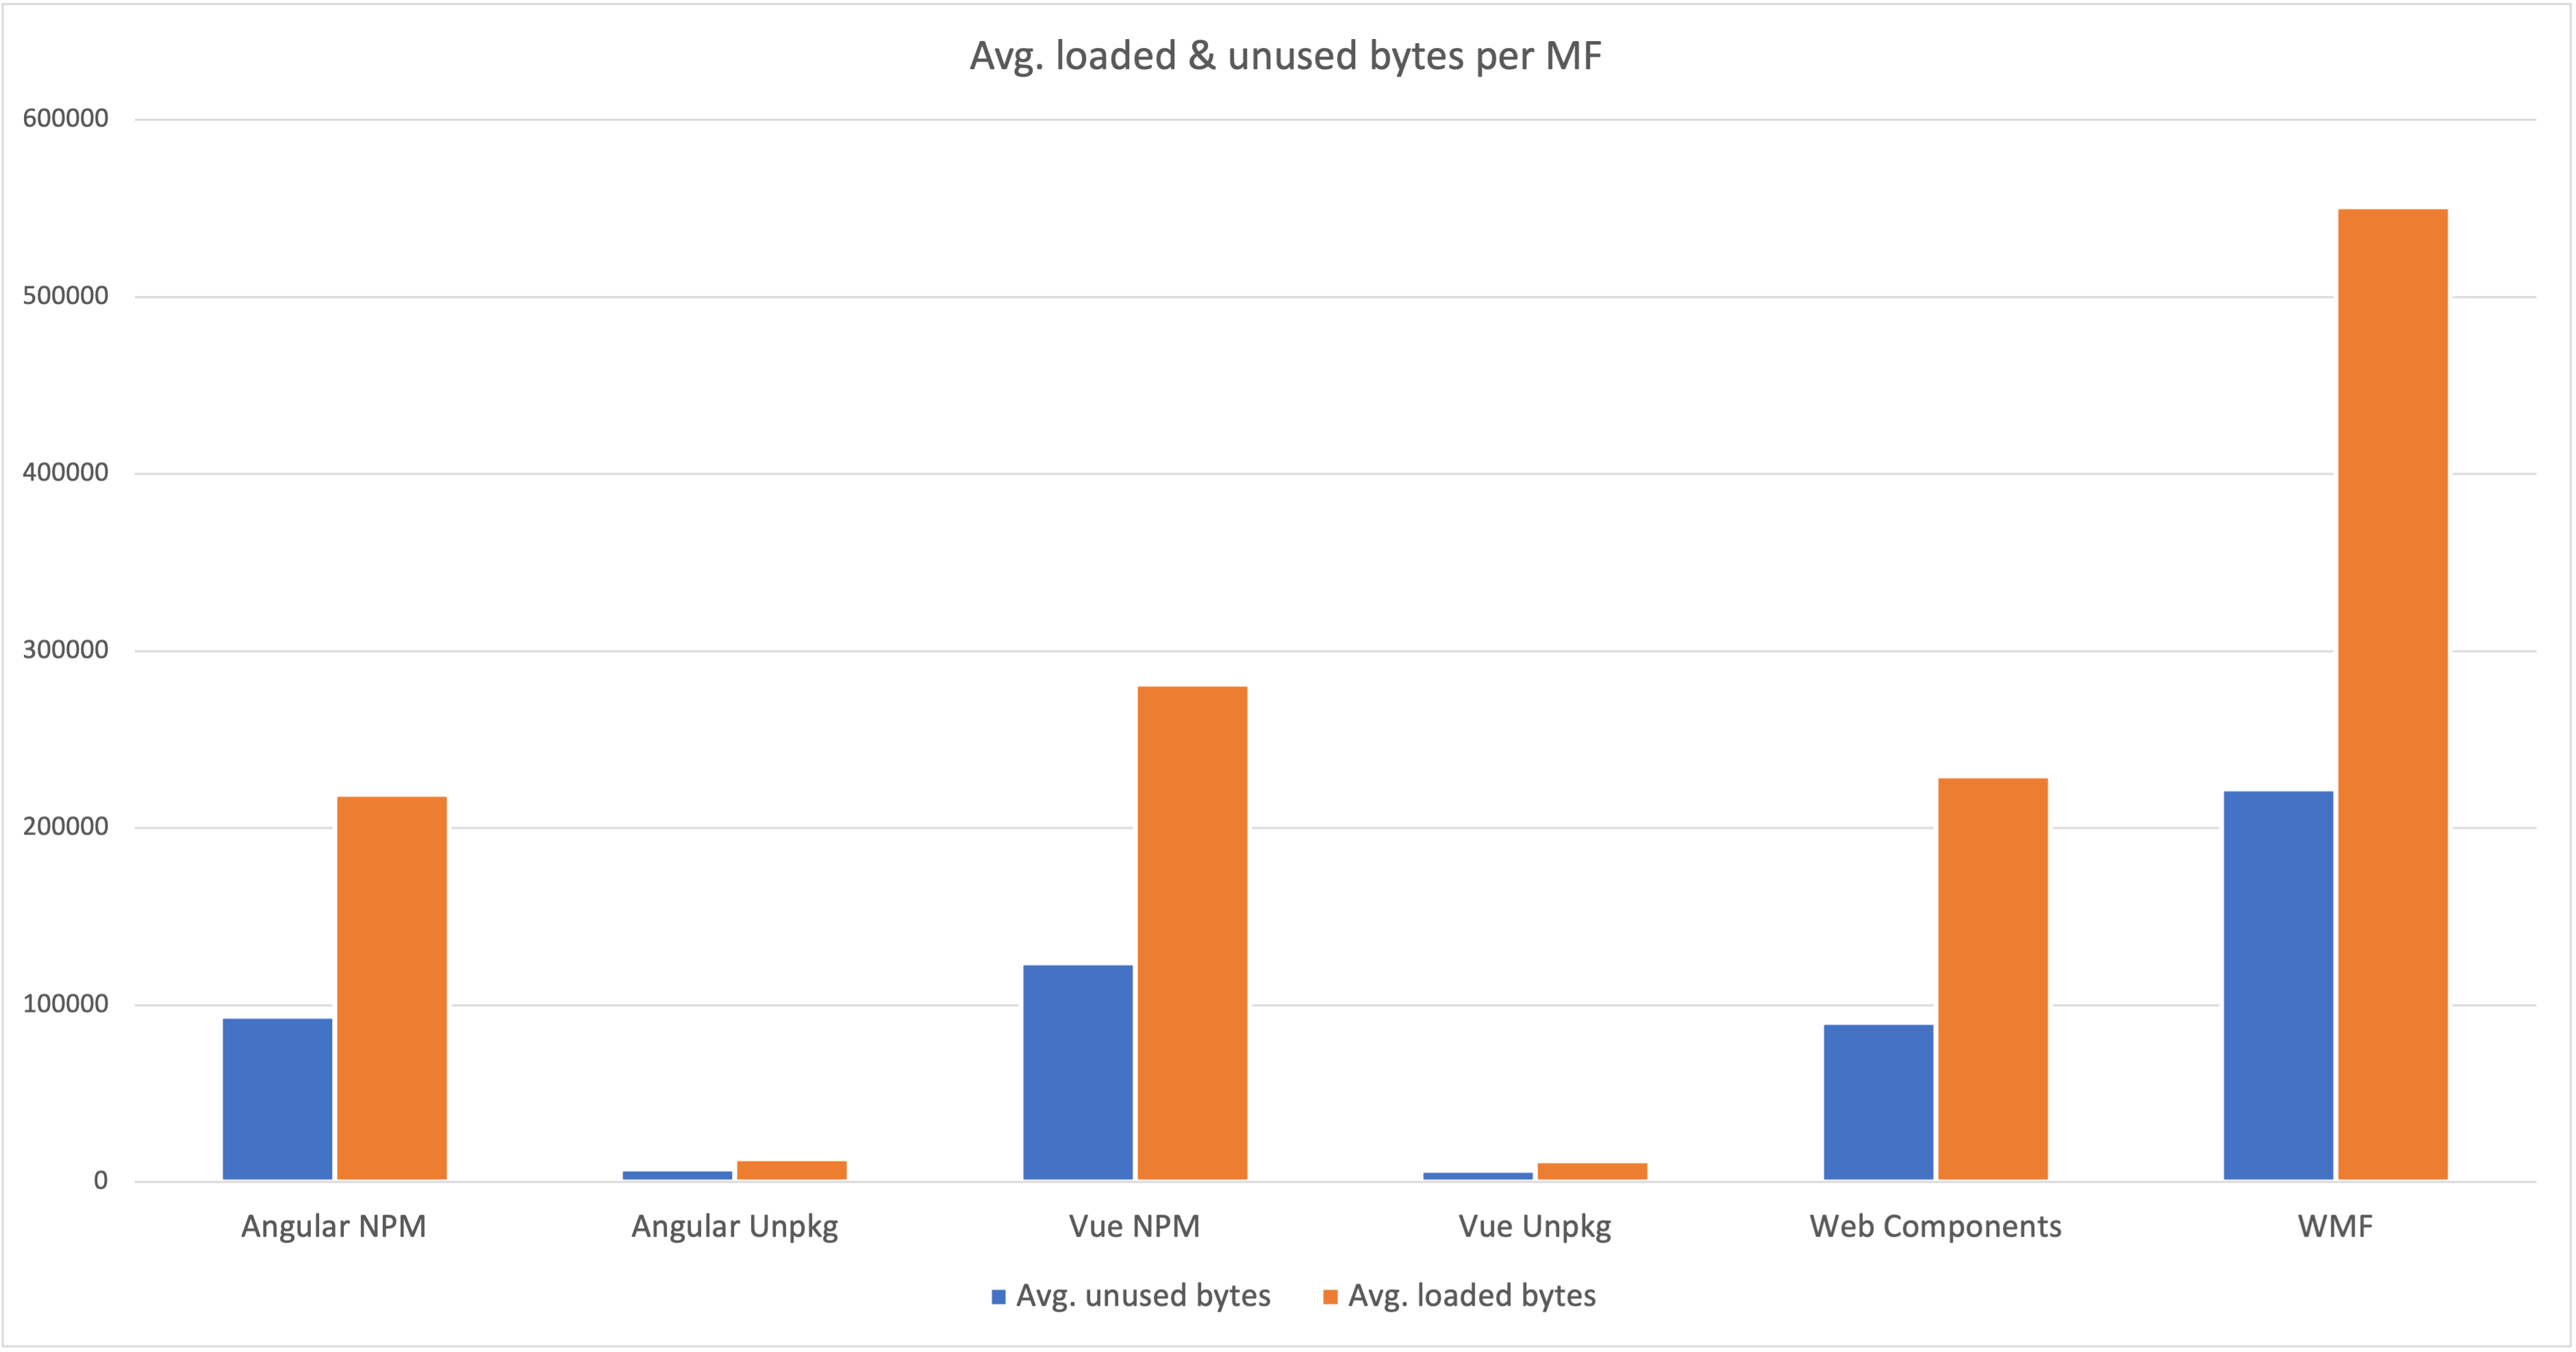
\includegraphics[width=1\textwidth]{Figures/avg_unsed_imported_1.png}
	\caption{Unused and imported bytes per landscape}
	\label{fig:unsed_imported_1}
\end{figure}

%\begin{figure}[!h]
%	\centering
%	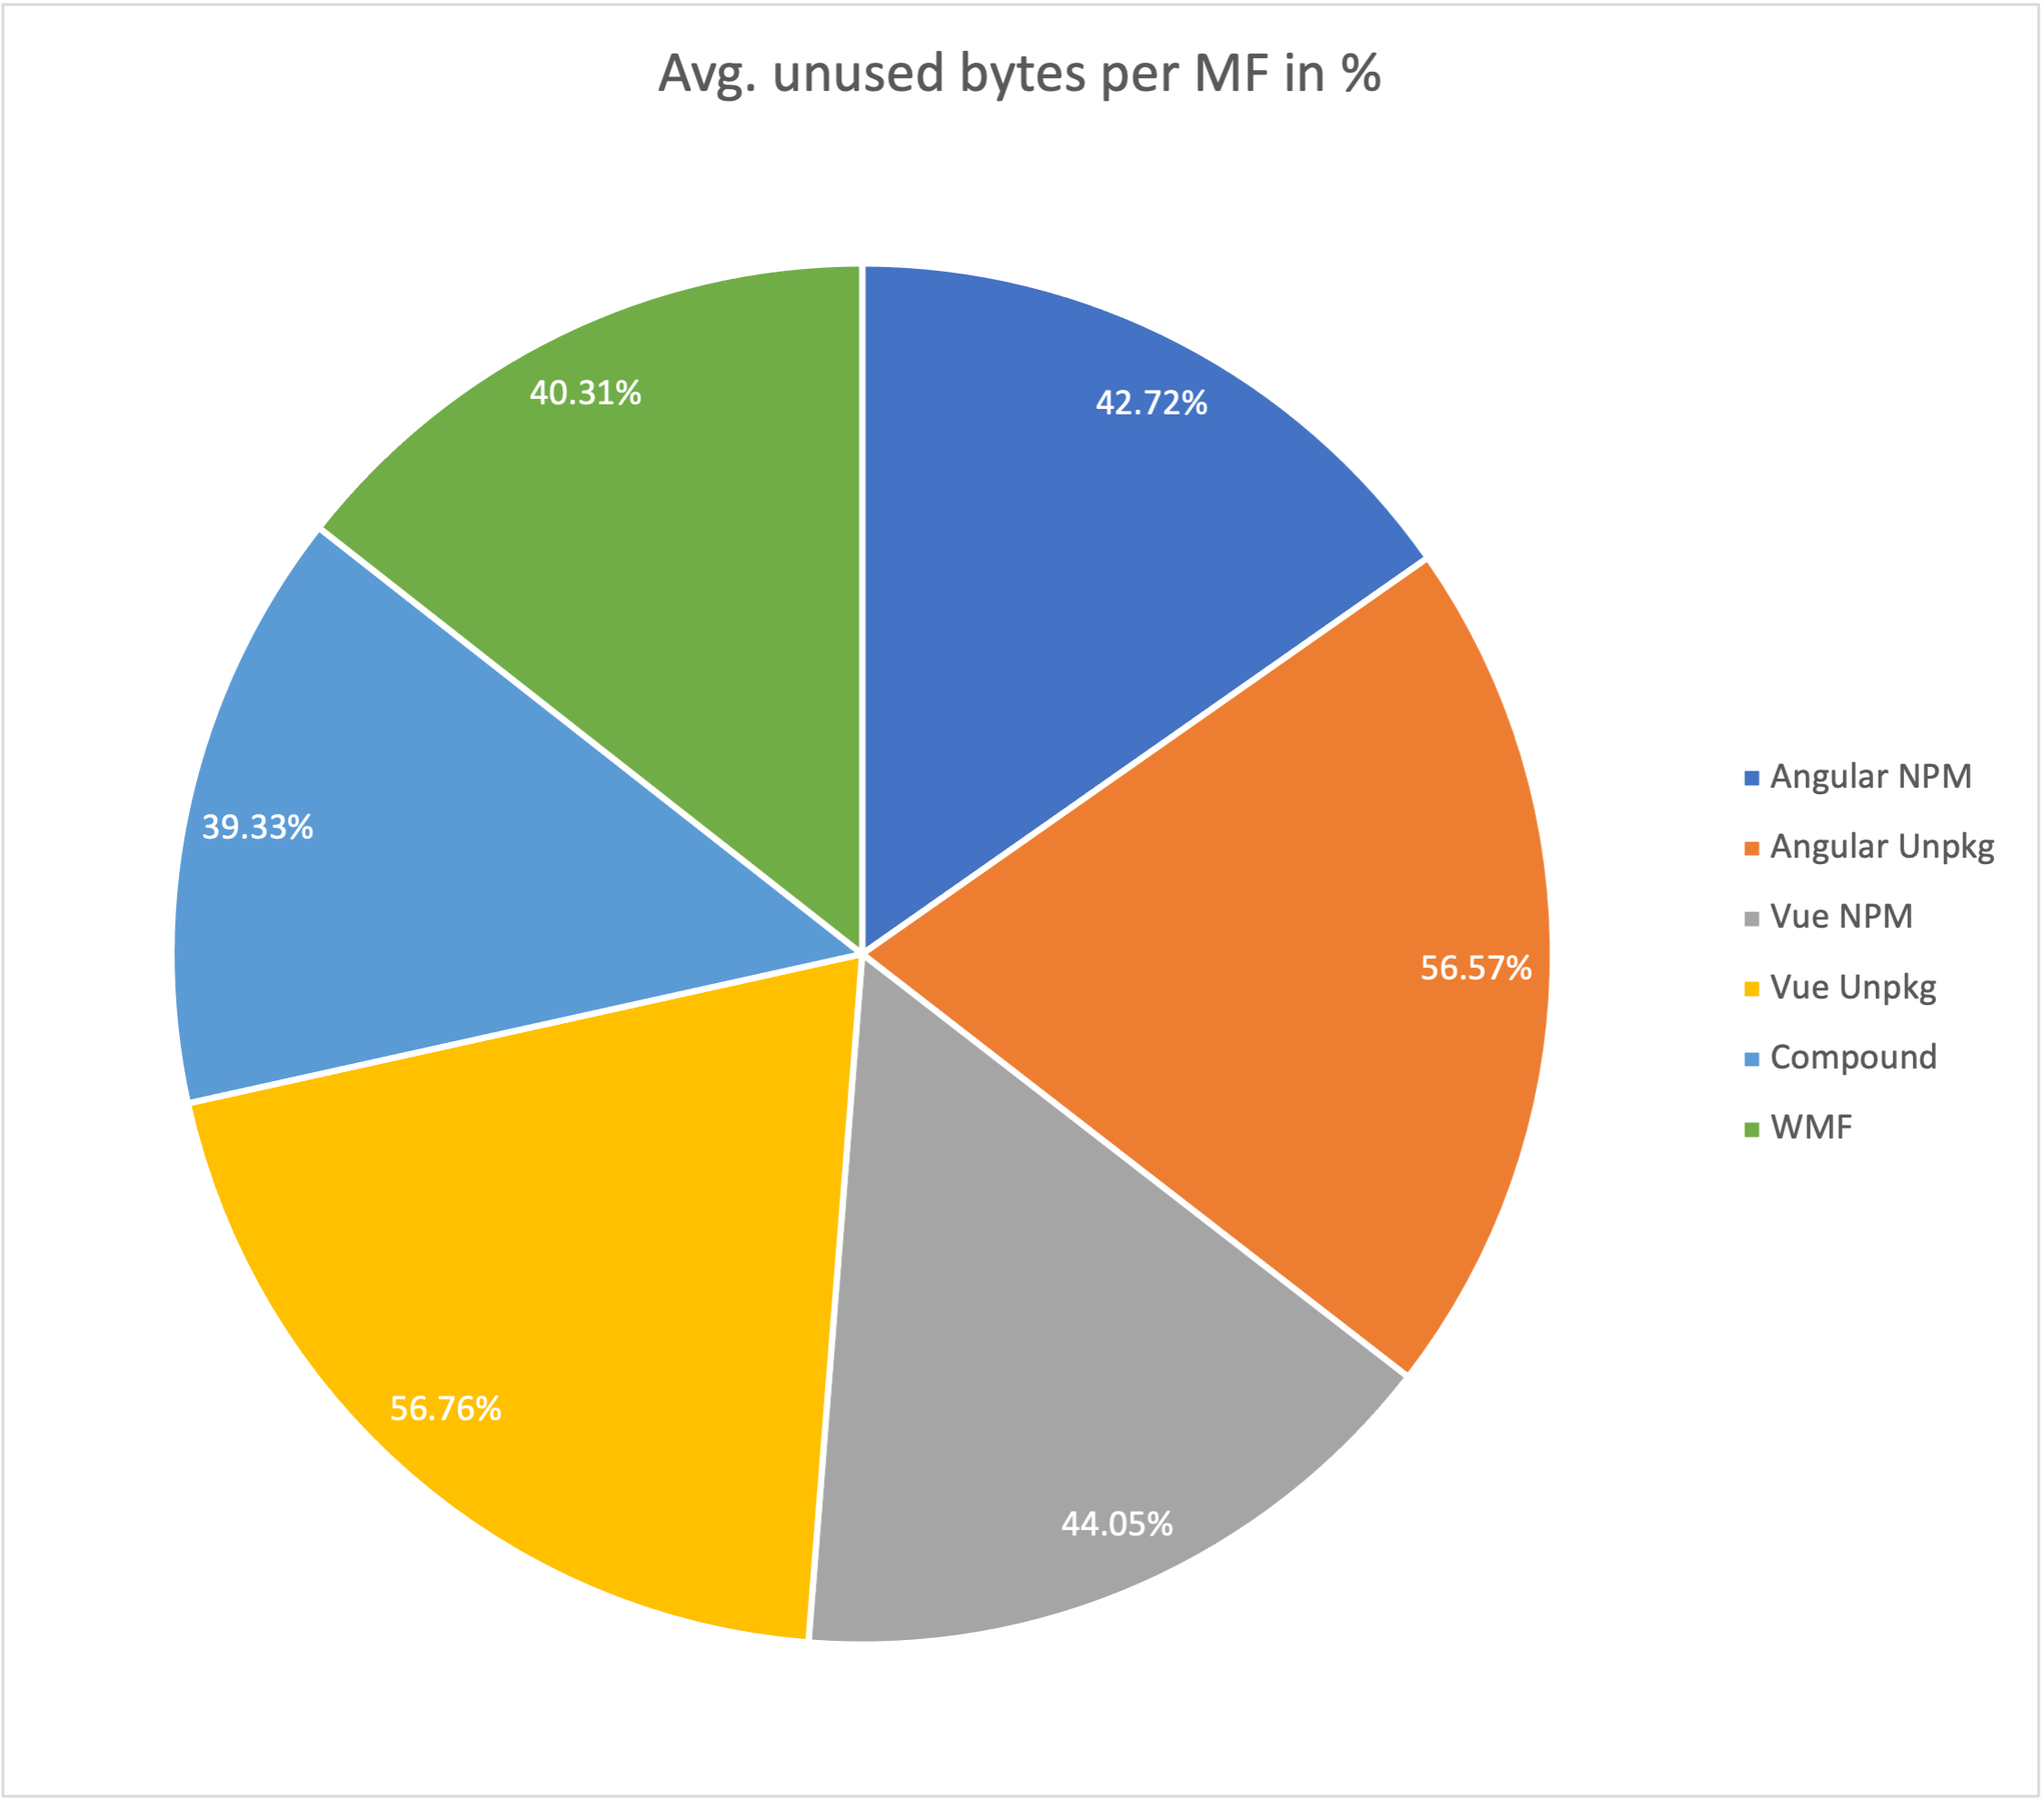
\includegraphics[width=1\textwidth]{Figures/avg_unsed_imported_2.png}
%	\caption{Unused and imported bytes per landscape in \%}
%	\label{fig:unsed_imported_2}
%\end{figure}

\normalsize
The shown data in table \ref{tab:lighthouse_used_report} and figure \ref{fig:unsed_imported_1} is highly application dependent. Still as these landscapes are considered to be generally representative, a display in efficiency can be drawn from the charts.
The Unpkg CDN landscapes show a low unused bytes ratio. Since only the required resources were requested from the CDN, only a few unused bytes were detected by the Lighthouse tool. 
For the WMF landscape, it can be argued, that due to the bundling with Webpack, a lot of bytes were imported but only a few of them were not used. This can be explained through how the Module Federation works, since every configured shared resource is checked if it should be shared or not.

The following chapter will be concluding the displayed data. Detailed tables and information can be found in the appendixes \ref{appendix1}, \ref{appendix2} and \ref{appendix3}.
